%\documentclass[11pt,a4paper,oneside,abstracton]{scrartcl}
\documentclass{article}

\usepackage[utf8]{inputenc}
\usepackage[ngerman]{babel} %fuer die deutsche Sprache
\usepackage{tabularx, multirow} %fuer Tabellen
\usepackage{booktabs}
\usepackage{tabularx,threeparttable,multicol}
\usepackage{pgfplots}
%\usepackage{graphicx, tikz} %Grafiken
\usepackage{amsmath, amssymb, amsthm} %einige hilfreiche Mathe-Pakete
\usepackage{mathtools}
\usepackage{verbatim}
\usepackage{epstopdf}
\usepackage{graphicx}
\usepackage{xcolor}
\usepackage{listings}
%\usepackage{todonotes} %zum Erstellen von To-Do-Listen
\usepackage{hyperref} %zur Verlinkung, Achtung: immer als letztes Paket laden!

% damit kann man die Seitenrand-Einstellungen  verwalten
% detaillierte Informationen finden sich in der Dokumentation zu KomaScript
%\KOMAoptions{BCOR=5mm} % gibt an, wieviel Platz links vom Text ist
%\KOMAoptions{DIV=13}   % rechnet aus, wieviel Platz der Text auf der Seite bekommt





\lstdefinelanguage{Julia}%
  {morekeywords={abstract,break,case,catch,const,continue,do,else,elseif,%
      end,export,false,for,function,immutable,import,importall,if,in,%
      macro,module,otherwise,quote,return,switch,true,try,type,typealias,%
      using,while},%
   sensitive=true,%
   alsoother={$},%$
   morecomment=[l]\#,%
   morecomment=[n]{\#=}{=\#},%
   morestring=[s]{"}{"},%
   morestring=[m]{'}{'},%
}[keywords,comments,strings]%

\lstset{%
    language         = Julia,
    basicstyle       = \ttfamily,
    keywordstyle     = \bfseries\color{blue},
    stringstyle      = \color{magenta},
    commentstyle     = \color{ForestGreen},
    showstringspaces = false,
}





%% Theoremumgebungen, die nuetzlich sein koennten:



%% Eckige Klammern: Theoreme kriegen vor ihre Zahl 
% noch die Section-Nummer
\newtheorem{theorem}{Theorem}[section] 
% eckige Klammern geben hier an, dass 
% sich alle Umgebungen hier denselben
% counter wie 'theorem' teilen
\newtheorem{lemma}[theorem]{Lemma}              
\newtheorem{proposition}[theorem]{Satz}
\newtheorem{definition}[theorem]{Definition}
\newtheorem{bemerkung}[theorem]{Bemerkung}
\newtheorem{beispiel}{Beispiel}
\newtheorem{algorithmus}[theorem]{Algorithmus}
\newtheorem{anm}[theorem]{Anmerkung}


\newtheoremstyle{case}{}{}{}{}{}{:}{ }{}
\theoremstyle{case}
\newtheorem{case}{Fall}

\newcommand*\rfrac[2]{{}^{#1}\!/_{#2}}
\newcommand{\cunderline}[2]{\textcolor{#1}{\textcolor{black}{#2}}}
\newsavebox\MBox
\newcommand\Cline[2][red]{{\sbox\MBox{$#2$}%
  \rlap{\usebox\MBox}\color{#1}\rule[-1.2\dp\MBox]{\wd\MBox}{0.5pt}}}

\newcommand{\EP}[3]{
\begin{center}
{\small 
\begin{tabularx}{0.97\columnwidth}{ll}
\toprule
\multicolumn{2}{c}{\textsc{#1}} \\
\midrule
\textbf{Gegeben:}& \parbox[t]{0.78\columnwidth}{#2\vspace*{1mm}} \\%[5mm]
\textbf{Frage:}& \parbox[t]{0.78\columnwidth}{#3\vspace*{.5mm}} \\ 
\bottomrule
\end{tabularx}
}
\end{center}
\medskip
}

\newcommand{\norm}[1]{\left\lVert#1\right\rVert}


\begin{document}
%
%\includegraphics[width=0.7\textwidth]{logo_claim_300dpi_cmyk_200.jpg}
%
\title{Das Schärfen von Bildern in Julia}
%
\author{Maximilian Simmoteit}
%
\date{\today}
%
\maketitle

%\pagebreak

%%%%
%\section*{Abstract}
%Bei gewichtete Wahlspielen handelt es sich um einfache Spiele, die kompakt darzustellen sind. In dieser Arbeit wird die Berechnungskomplexität der Entscheidung, ob verschiedene Eingriffe in ein Spiel die Macht erhöhen, untersucht.\newline
%Zu Beginn werden zwei Indices eingeführt, die die ``Macht'' eines Spielers in einem gewichteten Wahlspiel repräsentieren und Eigenschaften dieser untersuchen.\newline


%\section{Problem 1) Modellierung als Zylinder}

\section*{Grundannahmen dieser Arbeit}

In dieser Arbeit werden allgemeine Bilder als Funktionen $[0,1]^{2}\rightarrow [0,1]$ aufgefasst. Diskrete Bilder sind dann zweidimensionale Vektoren mit Werten in $[0,1]$. 


\section{Das Schärfen von Bildern}

In meinem Projekt habe ich mich damit beschäftigt den Algorithmus zum Schärfen von Bildern als Programm umzusetzen. Die Unschärfe eines Bildes wird hier als Faltung aufgefasst. Für einen Faltungskern $k$ und ein Bild $u$ ist das unscharfe Bild dann $k*u$. Für ein gegebenes unscharfe Bild $f$ ergibt sich daraus für die Optimierung der Minimierungsterm:
\begin{equation}
\min_{u\in U}\norm{k*u - f} + \alpha TV(u)
\end{equation}
oder für den diskreten Fall
\begin{equation}
min_{u\in U}\norm{k*u - f} + \alpha \norm{\lVert \nabla_{h} u \rVert_{2}}_{1}
\end{equation}
Zum Finden der optimalen Lösung $u$, kann man die Routine von Chambole-Pock nutzen. Als Eingabe benötigt diese einen Term der Form $\min_{x\in X} F(x) + G(Ax)$. Allerdings wird der Term für ein gefaltetes Bild dem nicht ganz gerecht, da dort auch im ersten Term noch eine Funktion auf die Variable angewandt wird. Deswegen setzt man $F(x) = 0$ und setzt den gesamten Term in $G(Ax)$ ein. Hier setzt man $Au = k*u$ und dementsprechend $A^{*}$ als dessen adjungierte Abbildung. Somit erhält man den folgenden Algorithmus:
\begin{align*}
x^{k+1} &= x^{k} - \tau (A^{*}y_{1}^{k} - div y_{2}^{k}) \\
\bar{x}^{k+1} &= 2\cdot x^{k+1} - x^{k} \\
y_{1}^{k+1} &= \frac{1}{1+\sigma} (y_{1}^{k} + \sigma\cdot A \bar{x}^{k+1} - \sigma\cdot f) \\
y{2}^{k+1} &= \frac{\alpha (y_{2}^{k+1} + \sigma \nabla \bar{x}^{k+1} )}{\max\{\alpha, \norm{y_{2}^{k+1} + \sigma \nabla \bar{x}^{k+1} }_{2}\}}
\end{align*}


\section{Umsetzung als Programm}
Und so wurde dieser Algorithmus als Programm umgesetzt.\newline
Zuerst betrachten wir, wie die Funktionen der diskreten Ableitung implementiert wurden.

\subsection{Der diskrete Gradient}

Um diesen Algorithmus zu implementieren muss man auch einen Algorithmus für den diskreten Gradienten implementieren. Für den diskreten Fall gilt allgemein, dass $(\nabla_{h} u)_{ijk} = ( \partial_{k}^{h,+} u)_{ij}$ für die vorwärts-Ableitung. Dieser Zusammenhang lässt sich in Julia sehr einfach umsetzen:
\begin{lstlisting}[language=Julia]
function disk_grad(u)
	return cat(disk_ab_v(u,1), disk_ab_v(u,2), dims=3)
end
\end{lstlisting}
für eine Funktion "disk ab v", die hier die diskrete vorwärts-Ableitung liefert. Das Argument "dims=3" besagt, dass die beiden zweidimensionalen Arrays zu einem dreidimensionalen zusammengefügt werden. Die diskrete vorwärts-Ableitung lässt sich mit einer einfachen Übertragung und Iteration über alle Elemente implementieren:
\begin{lstlisting}[language=Julia]
function disk_ab_v(u::Array{Float64,2}, k::Int)
	n = size(u,1)
	m = size(u,2)
	h = 1/sqrt(n*m)
	v = zeros((n,m))
	if k == 1
		for i = 1:n
			for j = 1:m
				if i < n
					v[i, j] = (u[i+1, j] - u[i,j])/h
				else
					v[i, j] = 0
				end
			end
		end
	elseif k == 2
		for i = 1:n
			for j = 1:m
				if j < m
					v[i, j] = (u[i, j+1] - u[i,j])/h
				else
					v[i, j] = 0
				end
			end
		end
	else

	end
	return v
end
\end{lstlisting}



\subsection*{Performance Verbesserungen}

Diese Implementierung ist sehr direkt dem Lehrbuch entnommen und noch nicht für die Performance eines Computers optimiert. Als erstes, kann man "Type Annotations" einführen. Dies sagt der Programmiersrache, welche Datentypen man erwartet und erleichtert das Optimieren und kompilieren dieses Codes:
\begin{lstlisting}[language=Julia]
function disk_ab_v(u::Array{Float64,2}, k::Int)
...
function disk_grad(u::Array{Float64,2})
...
\end{lstlisting}
Als nächstes merkt man, dass die Schleifenschritte voneinander unabhängig sind (von u wird nur gelesen und v wird nur beschrieben) und man kann dieser Schleife das Makro @simd vorstellen. Dies kann bei vielen Prozessoren zu schnellerer Ausführung führen. Allerdings kann man das nur bei der innersten Schleife anführen, da eine einfache Instruktion auf verschiedene Daten angewandt werden kann. Um das zu verbessern, kann man die zwei Schleifen zu einer Schleife zusammen fassen. Da ich diesen Algorithmus schon mehrfach getestet habe, kann Julia darauf verzichten sogenannte "BoundsChecks" durchzuführen, mittels des @inbounds Makros.
\begin{lstlisting}[language=Julia]
M = n*m
@simd for a = 0:M-1
		j = a % m +1
		i = a (ganzzahlige Division) m +1
		if i < n
			@inbounds v[i, j] = (u[i+1, j] - u[i,j])/h
		else
			@inbounds v[i, j] = 0
		end
end
\end{lstlisting}
Da für $k$ nur zwei Fälle möglich sind, kann man die if-else Verzweigung sein lassen und für die beiden vorwärts-Ableitungen eigene Funktionen schreiben.
Zuletzt kann noch der Speicher verbessert werden. Bisher wurde bei jedem Aufruf, mittels $v=zeros((n,m))$, neuer Speicher vom Betriebssystem angefordert. Da in der Optimierungsschleife diese Funktion nur jeweils einmal aufgerufen wird und das Ergebnis danach nicht mehr benötigt, kann man ein Array definieren, das man in jedem Schleifendurchlauf neu beschreibt. Dies macht man folgendermaßen:
\begin{lstlisting}[language=Julia]
function perf_disk_grad(u::Array{Float64,2}, res_arr::Array{Float64,3})
	perf_disk_ab_v_1(u,res_arr)
	perf_disk_ab_v_2(u,res_arr)
end
...
function perf_disk_ab_v_1(u::Array{Float64,2},v::Array{Float64,3})
...
	if i < n
		@inbounds v[i, j, 1] = (u[i+1, j] - u[i,j])/h
	else
		@inbounds v[i, j, 1] = 0
	end
...
end
...
\end{lstlisting}
hier ist "res arr" ein Array in den Dimensionen der Ausgabe. Das Array wird den Funktionen jeweils übergeben "perf disk ab v 1" beschreibt die Werte $v[i,j,1]$ und "perf disk ab v 2" beschreibt die Werte $v[i,j,2]$.


\subsection{Die diskrete Divergenz}
Bei der diskreten Divergenz werden die Ergebnisse diskreten rückwärts-Ableitung miteinander addiert. Programmiert sieht das so aus:
\begin{lstlisting}[language=Julia]
function disk_div(u)
	return disk_ab_r(u[:,:,1],1) + disk_ab_r(u[:,:,2],2)
end
\end{lstlisting}
Die diskrete rückwärts-Ableitung lässt sich mithilfe von Schleifen auch ganz leicht nach Julia übertragen:
\begin{lstlisting}[language=Julia]
function disk_ab_r(u::Array{Float64,2}, k::Int)
	n = size(u,1)
	m = size(u,2)
	h = 1/sqrt(n*m)
	v = zeros((n,m))
	if k == 1
		for i = 1:n
			for j = 1:m
				if i == 1
					v[i,j] = u[i,j]/h
				elseif i < n
					v[i, j] = (u[i, j] - u[i-1,j])/h
				else
					v[i, j] = -u[n-1,j]/h
				end
			end
		end
	elseif k == 2
		for i = 1:n
			for j = 1:m
				if j == 1
					v[i,j] = u[i,j]/h
				elseif j < m
					v[i, j] = (u[i, j] - u[i,j-1])/h
				else
					v[i, j] = -u[i,m-1]/h
				end
			end
		end
	else

	end
	return v
end
\end{lstlisting}


\subsection*{Performance Verbesserungen}
Auch hier ist das nur eine simple Übertragung in Julia. Wie in den vorherigen Verbesserungen kann man mittels inbounds und simd Makros die Performance verbessern. Die Verbesserung der Speichernutzung funktioniert hier allerdings etwas anders.


\subsection{Die diskrete Faltung}

Bei der diskreten Faltung wird ein Bild der Dimension $n\times m$ mit einem Vektor der Dimension $(2r+1)\times (2s+1)$ gefaltet. Da Arrays in Julia mit Index $1$ anfangen, habe ich das Array zum Falten als Funktion modelliert:
\begin{lstlisting}[language=Julia]
function kreis_k(h,p,q,r,s)
	if p^2/r^2 + q^2/s^2 <= 1
		return h
	else
		return 0
	end
end
\end{lstlisting}
Damit lässt sich die diskrete Faltung wie folgt programmieren:
\begin{lstlisting}[language=Julia]
function disk_falt(u::Array{Float64,2}, r::Int, s::Int,
	k::Function,h::Float64)
	n_d = size(u,1)
	m_d = size(u,2)
	A = zeros((n_d-2*r, m_d-2*s))
	for i = 1:n_d-2*r
		for j = 1:m_d-2*s
			a = 0
			for n = i-r:i+r
			for m = j-s:j+s
				a = a + u[n+r, m+s]*k(h,i-n,j-m,r,s)
			end
			end
			A[i,j] = a
		end
	end
	return A
end
\end{lstlisting}
Hierbei wird die Rückgabe $h$ des Faltungskerns der Faltungsfunktion übergeben. In der Hauptschleife wird einmal die Zahl aller Felder berechnet, in denen der Faltungskern nicht Null ist und der Kehrwert als $h$ an die Funktionen gegeben, damit die Summe über $k$ $1$ ergibt.\newline
Zuletzt fehlt noch die adjungierte Faltung. Die akzeptiert ein Array der Dimension $n\times m$ und gibt ein Array der Dimension $(n+2r)\times (m+2s)$ aus. Die adjungierte Faltung lässt sich wie folgt programmieren:
\begin{lstlisting}[language=Julia]
function disk_falt_adj(w::Array{Float64,2}, r::Int, s::Int,
	k::Function,h::Float64)
	n_a = size(w,1)
	m_a = size(w,2)
	A = zeros((n_a + 2*r, m_a + 2*s))
	for i = 1:n_a+2*r
	for j = 1:m_a+2*s
		a = 0
		for n = max(1,i-2*r):min(i, n_a)
		for m = max(1,j-2*s):min(j, m_a)
			a = a + w[n, m]*k(h,n-i+r,m-j+s,r,s)			
		end
		end
		A[i,j] = a
	end
	end
	return A
end
\end{lstlisting}
Dass das wirklich die adjungierte Faltung ist lässt sich mit folgendem Programm überprüfen:
\begin{lstlisting}[language=Julia]
function dual_paarung(u::Array{Float64,2}, w::Array{Float64,2})
	n1 = size(u,1)
	n2 = size(u,2)
	a = 0

	for i=1:n1
		for j=1:n2
			a = a + u[i, j]*w[i, j]
		end
	end

	return a

end

function teste_adj_faltung(n_wert,m_wert,r_wert,s_wert, k)
	f = 0
	for r=1:r_wert
		println("r: ",r)
		for s=1:s_wert
			for n = (n_wert-10):n_wert
				for m = (m_wert-10):m_wert
				u = rand(Float64,(n,m))
				w = rand(Float64,(n-2*r,m-2*s))
				res1 = dual_paarung(w, 
				 disk_falt(u,r,s,k))
				res2 = dual_paarung(
				 disk_falt_adj(w,r,s,k),u)
				if abs(res1-res2) > 1e-4
					println("!Fehler: ", 
					 res1, ", ", res2)
					f = f+1
				end
				end
			end
		end
	end
	return f
end
\end{lstlisting}


\subsection*{Performance Verbesserungen}
Bei der Faltung und der adjungierten Faltung handelt es sich um die Flaschenhälse dieser Berechnung. Deshalb kann es sich lohnen diese Berechnung zu parallelisieren. Durch das threads Makro am Anfang der Schleifen:
\begin{lstlisting}[language=Julia]
...
@threads for i = 1:n_d-2*r
...
\end{lstlisting}
werden die $n_d -2\cdot r$ Schleifendurchläufe auf die Threads der Julia-Umgebung aufgeteilt. Vor dem Starten von Julia kann man mittels
\begin{lstlisting}[language=Bash]
export JULIA_NUM_THREADS=8
\end{lstlisting}
Julia mehrere Threads zuweisen und so die Ausführung beschleunigen.\newline
Ebenso wie bei der diskreten Divergenz und dem diskreten Gradienten lassen sich hier schon die Ergebnis Arrays übergeben, so dass keine neuen Speicherbelegungen stattfinden.  


\subsection{Die Optimierungsschleife}

Zuerst müssen verschiedene Werte initialisiert werden:
\begin{lstlisting}[language=Julia]
function perf_bild_schaerfer(bild::Array{Float64,2}, alpha::Float64,
	r::Int,  s::Int, k::Function; it=10000, sigma=-1.0, tau=-1.0)
	
	n_a = size(bild,1)
	m_a = size(bild,2)

	n = n_a + 2*r
	m = m_a + 2*s

	xk = embed_image(bild,r,s)
	y1k = zeros((n_a,m_a))
	y2k = zeros((n,m,2))

	div_y2k = zeros((n,m))
	grad_xk3 = zeros((n,m,2))

	falt_adj_y1k = zeros((n,m))
	falt_xk3 = zeros((n_a, m_a))
	sum_y2k2 = zeros((n,m,2))

	xk2 = zeros((n,m))
	xk3 = zeros((n,m))
	y1k2 = zeros((n_a,m_a))
	y2k2 = zeros((n,m,2))

	if sigma < 0 || sigma*tau >= 1/(n*m*8)
		sigma = (1/(sqrt(n)*sqrt(m)*sqrt(8)+1))
	end
	if tau < 0 || sigma*tau >= 1/(n*m*8)
		tau = 1/(sqrt(n)*sqrt(m)*sqrt(8)+1)
	end
	
	ret_d_falt_kerns = 1/check_number(k,r,s)
\end{lstlisting}
$xk$ steht hier für $x^{k}$ und $y1k$ für $y_{1}^{k}$ sowie $y2k$ für $y_{2}^{k}$. $y$ wird als $0$ initialisiert und $x$ als das Eingabebild, bei dem die Ränder mit Nullen aufgefüllt sind. $\sigma$ und $\tau$ sind so gewählt, dass $\sigma\cdot \tau < \frac{1}{h^{2}\cdot 8}$. Damit lässt sich nun die Optimierungsschleife umsetzen. Hierbei wird jeweils $xk2, y1k2,y2k2$ für $x^{k+1}$ geschrieben. Der erste Schritt des Algorithmus
\[
x^{k+1} = x^{k} - \tau (A^{*}y_{1}^{k} - div y_{2}^{k})
\]
lässt sich somit als
\begin{lstlisting}[language=Julia]
	perf_disk_div(y2k, div_y2k)
	perf_disk_falt_adj(y1k,r,s,k, ret_d_falt_kerns,falt_adj_y1k)
	@. @inbounds xk2 = xk - tau*(falt_adj_y1k - div_y2k)
\end{lstlisting}
schreiben.
Hierbei wird durch das @. Makro eine komponentenweise Berechnung erwirkt. Dadurch wird wird das Ergebnis direkt in xk2 gespeichert und kein Speicher wird belegt.\newline
Der zweite Schritt
\[
\bar{x}^{k+1} = 2\cdot x^{k+1} - x^{k}
\]
ist ganz einfach
\begin{lstlisting}[language=Julia]
	@. @inbounds xk3 = 2.0 *xk2 - xk
\end{lstlisting}
und die letzten beiden Schritte
\begin{align*}
y_{1}^{k+1} &= \frac{1}{1+\sigma} (y_{1}^{k} + \sigma\cdot A \bar{x}^{k+1} - \sigma\cdot f) \\
y{2}^{k+1} &= \frac{\alpha (y_{2}^{k+1} + \sigma \nabla \bar{x}^{k+1} )}{\max\{\alpha, \norm{y_{2}^{k+1} + \sigma \nabla \bar{x}^{k+1} }_{2}\}}
\end{align*}
lassen sich als
\begin{lstlisting}[language=Julia]
	perf_disk_falt(xk3,r,s,k, ret_d_falt_kerns,falt_xk3)
	@. @inbounds y1k2 = (1.0 /(1.0 +sigma))*
			(y1k + sigma*falt_xk3 - sigma*bild)
			
	perf_disk_grad(xk3, grad_xk3)
	@. @inbounds sum_y2k2 = y2k + sigma*grad_xk3
	prox_g(sum_y2k2,alpha,y2k2)
\end{lstlisting}
programmieren. Hierbei ist prox g folgende Funktion:
\begin{lstlisting}[language=Julia]
function prox_g(inp::Array{Float64,3}, alpha, val::Array{Float64,3})
n = size(inp,1)
m = size(inp,2)

for i = 1:n
for j = 1:m
	@inbounds val[i,j,1] =
	 alpha*inp[i,j,1]/max(alpha, sqrt(inp[i,j,1]^2 + inp[i,j,2]^2))

	@inbounds val[i,j,2] =
	 alpha*inp[i,j,2]/max(alpha, sqrt(inp[i,j,1]^2 + inp[i,j,2]^2))
end
end
end

\end{lstlisting}

Zuletzt müssen die neuen Variablen die alten überschreiben und die Schleife ist fertig:
\begin{lstlisting}[language=Julia]
	xk = xk3
	y1k = y1k2
	y2k = y2k2)
\end{lstlisting}
Aufgrund der kleinen Schrittgrößen läuft dieses Programm eine fest vorgegebene Schrittzahl durch.
\newline
Von der Konsole kann man dieses Programm wie folgt aufrufen:
\begin{lstlisting}[language=bash]
julia src/run_script.jl --i "exp_bilder/test_bild1_falt.png" --vr 3
--hr 3 --a 5.0 --it 15000
\end{lstlisting}
\newpage


\section{Anwendung an einem Beispielbild}

%\begin{figure}
%  \includegraphics[width=\linewidth]{boat.jpg}
%  \caption{A boat.}
%  \label{fig:boat1}
%\end{figure}

%Figure \ref{fig:boat1} shows a boat.

Unser ursprüngliches Eingabebild ist: ~\ref{fig:bild1}
\begin{figure}
  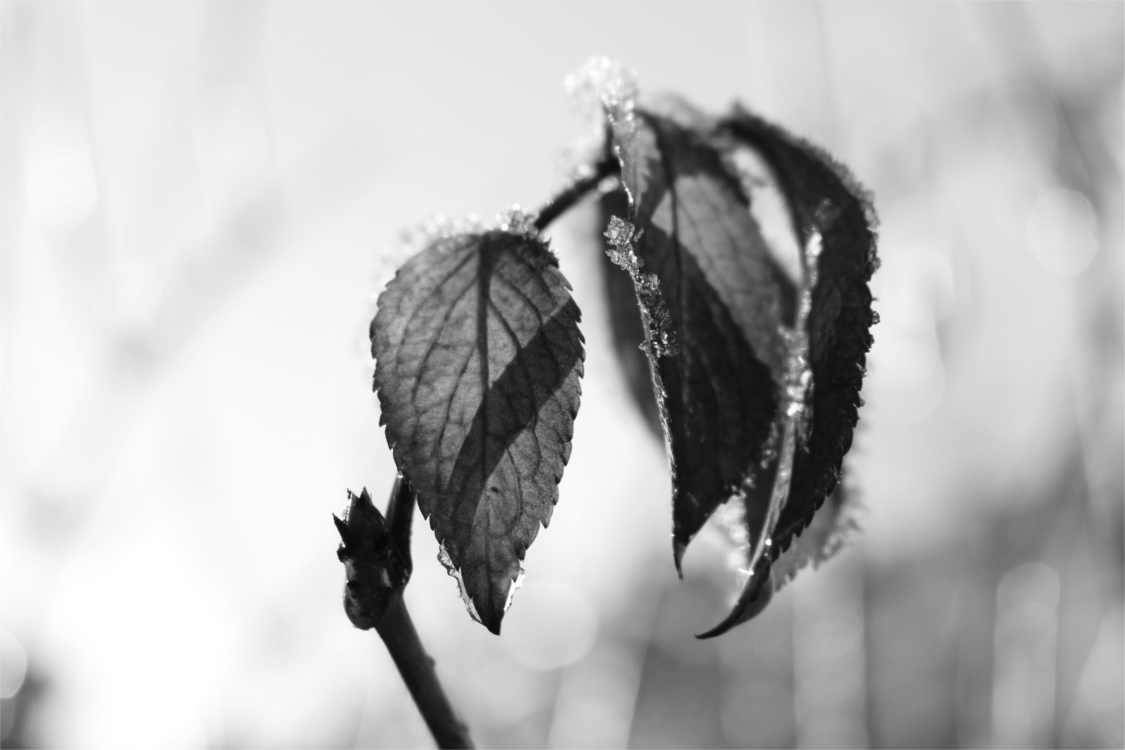
\includegraphics[width=\linewidth]{../output/input2.png}
  \caption{Das ursprüngliche Bild}
  \label{fig:bild1}
\end{figure}

dieses Bild ist schon scharf. Damit die Anwendung unseres Algorithmus' Sinn macht brauchen wir ein unscharfes Bild. Hierzu wird unser Eingabebild mit unserem Faltungskern gefaltet. Als Beispiel wurde es mit $r=3,\,s=3$ gefaltet:

\begin{figure}
  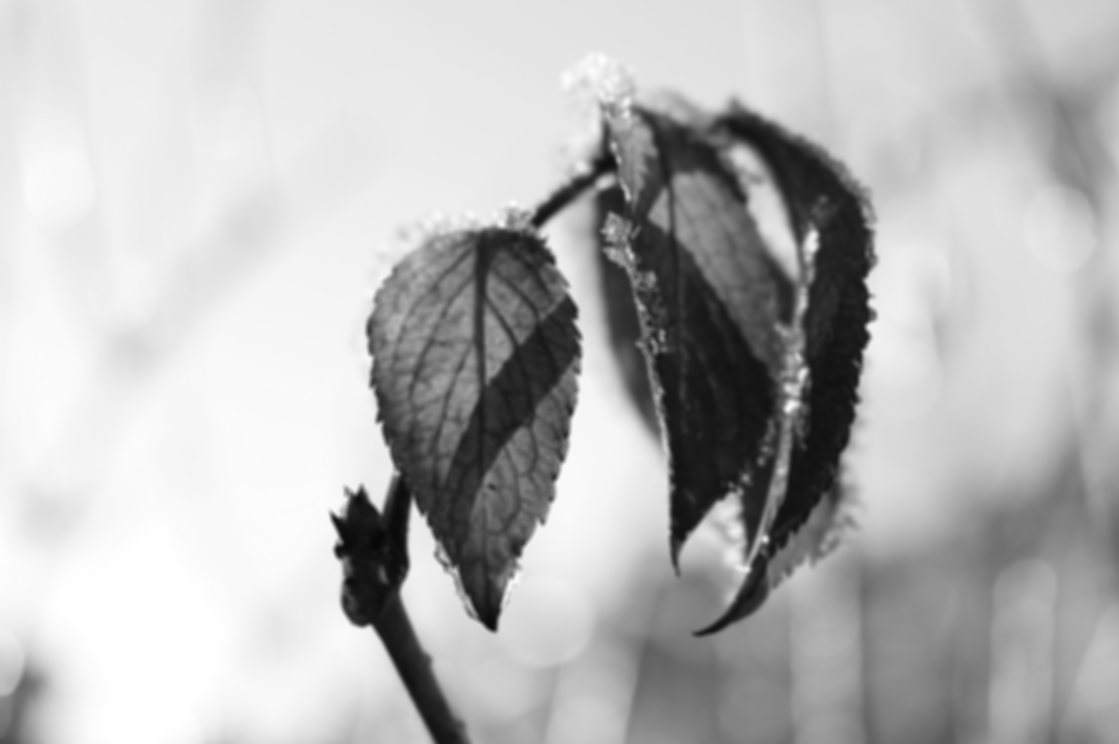
\includegraphics[width=\linewidth]{../output/input2_gefaltet2.png}
  \caption{Das ursprüngliche Bild gefaltet}
  \label{fig:bildg2}
\end{figure}

Im Folgenden wurde der Algorithmus mit verschiedenen $\alpha$-Werten und jeweils $18000$ Schritten, $\sigma=\tau=\frac{1}{nm\sqrt{8}+1}$ ausgeführt:

\begin{figure}
  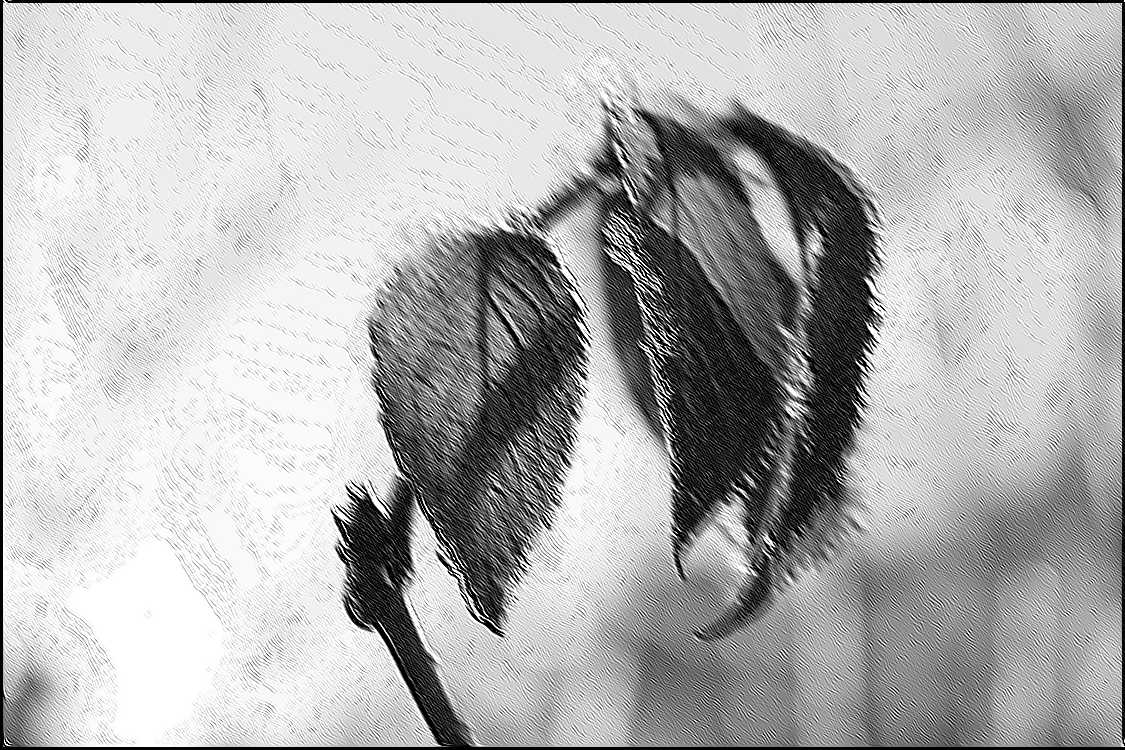
\includegraphics[width=\linewidth]{../output/neu2_output_18k_alpha1.png}
  \caption{$\alpha=1$}
  \label{fig:bilda1}
\end{figure}

\begin{figure}
  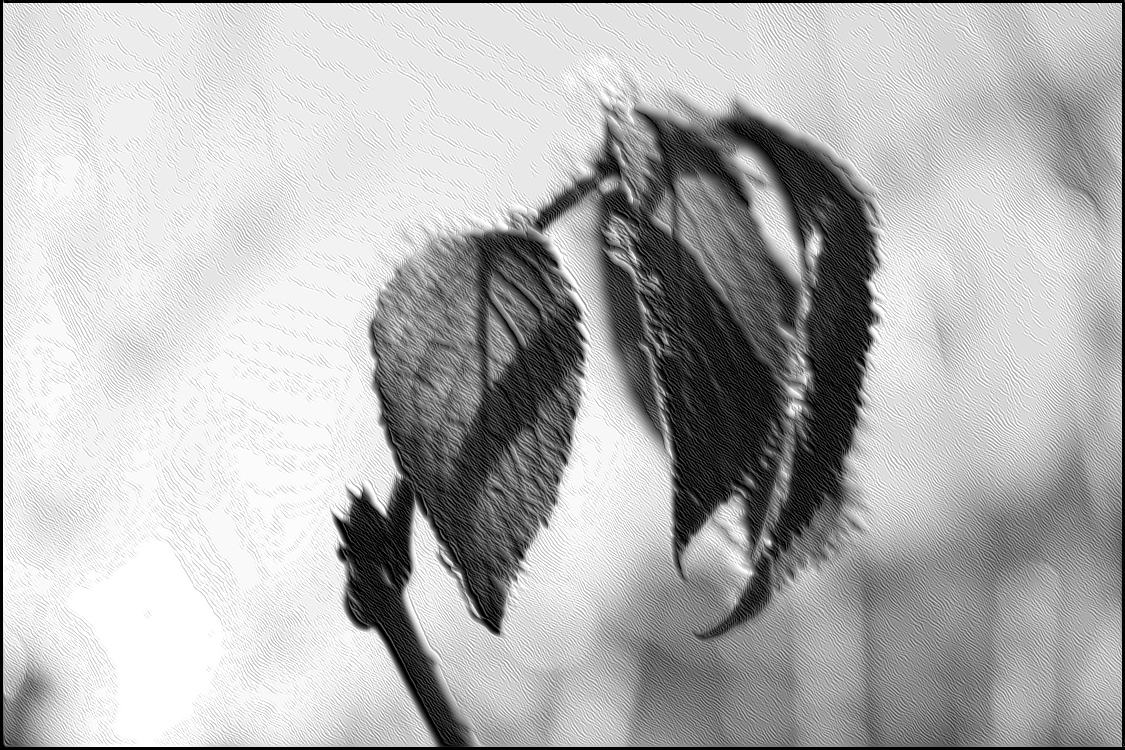
\includegraphics[width=\linewidth]{../output/neu2_output_18k_alpha01.png}
  \caption{$\alpha=0.1$}
  \label{fig:bilda2}
\end{figure}

\begin{figure}
  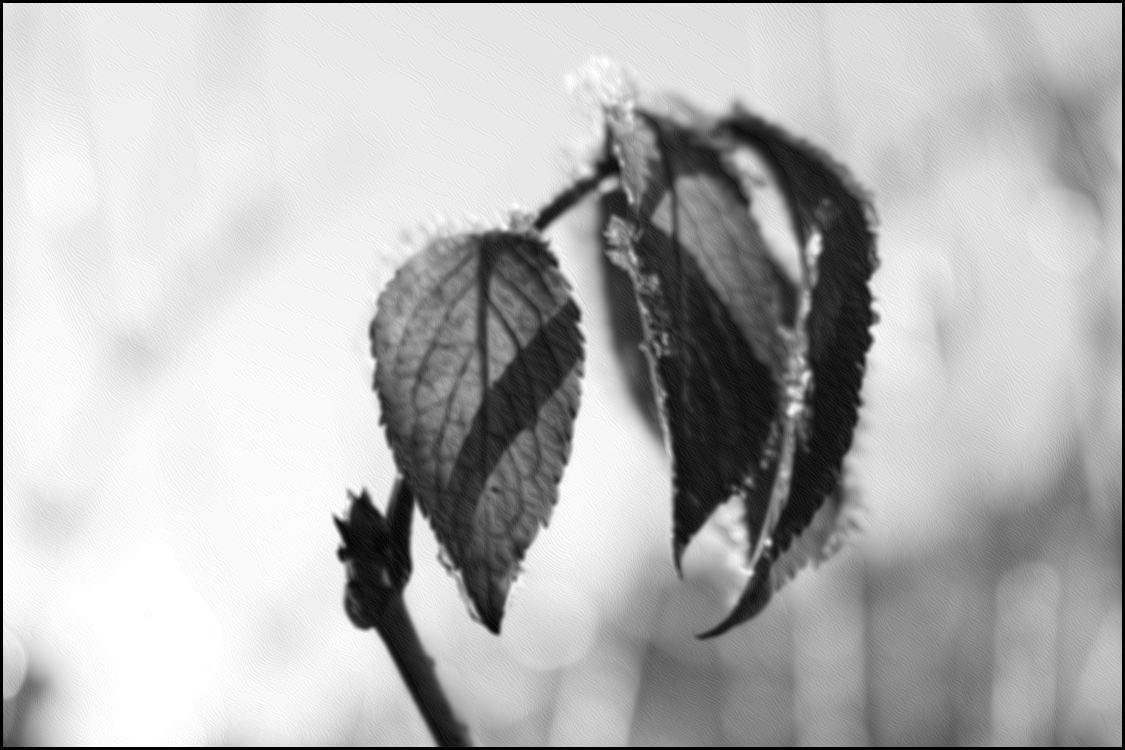
\includegraphics[width=\linewidth]{../output/neu2_output_18k_alpha001.png}
  \caption{$\alpha=0.01$}
  \label{fig:bilda3}
\end{figure}

\begin{figure}
  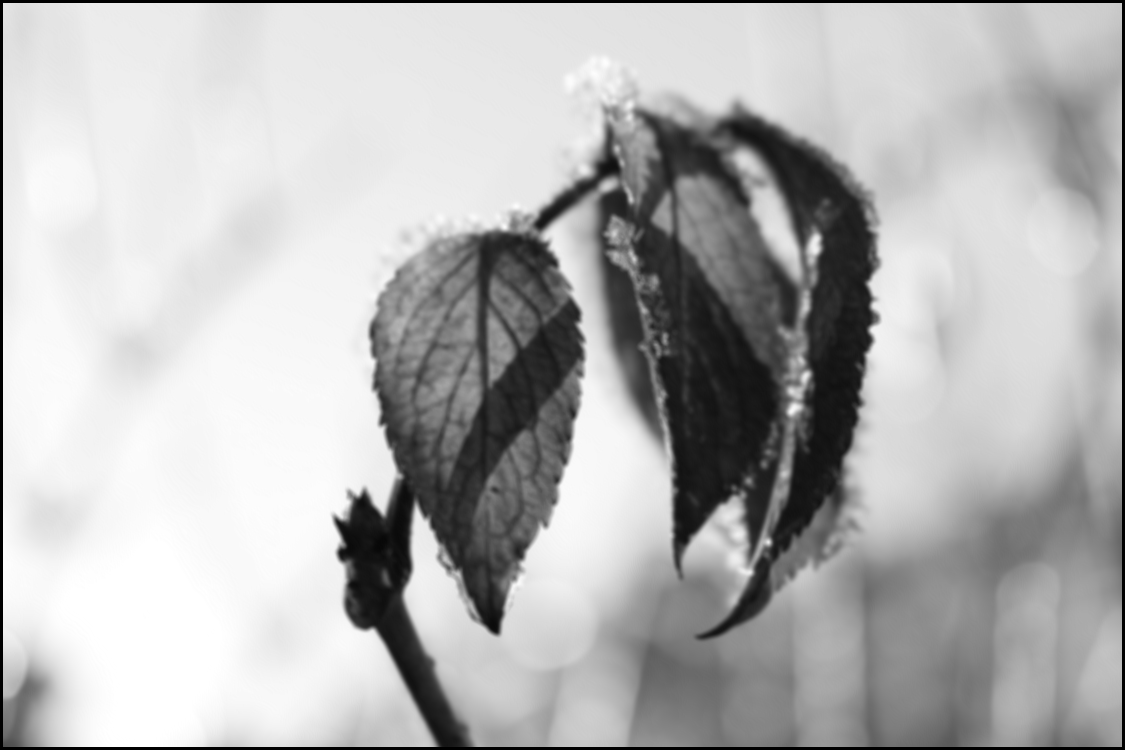
\includegraphics[width=\linewidth]{../output/neu2_output_18k_alpha0001.png}
  \caption{$\alpha=0.001$}
  \label{fig:bilda4}
\end{figure}

\begin{figure}
  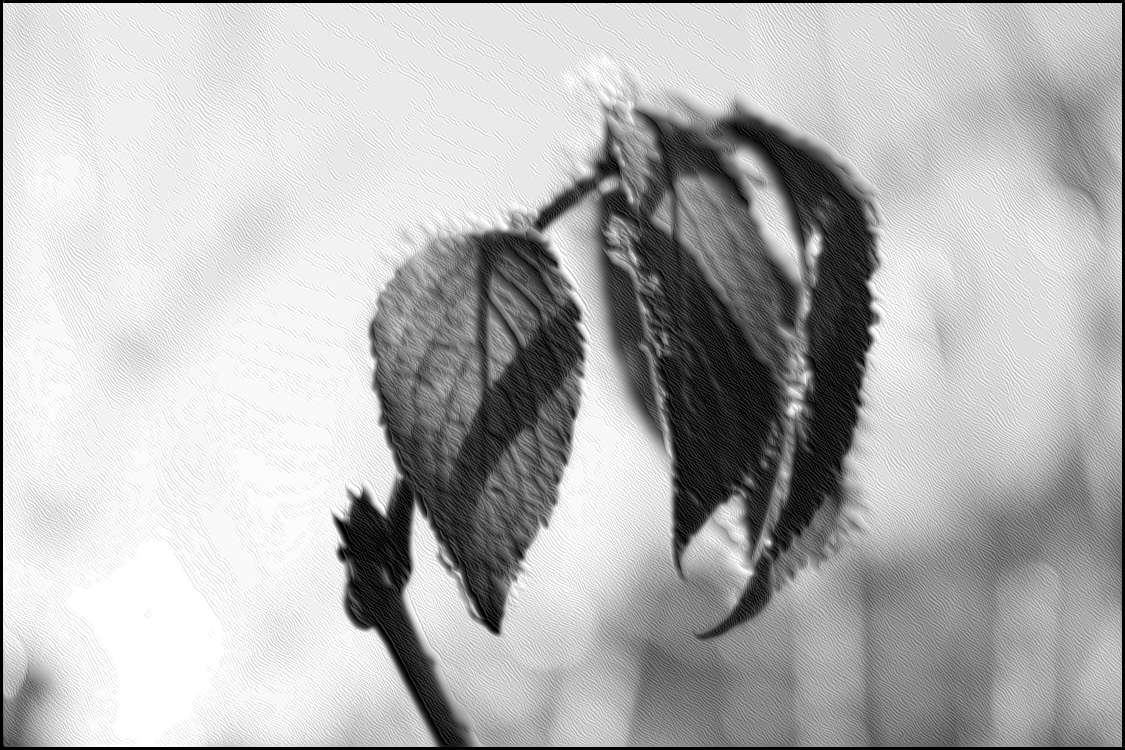
\includegraphics[width=\linewidth]{../output/neu2_output_18k_alpha005.png}
  \caption{$\alpha=0.05$}
  \label{fig:bilda5}
\end{figure}

\begin{figure}
  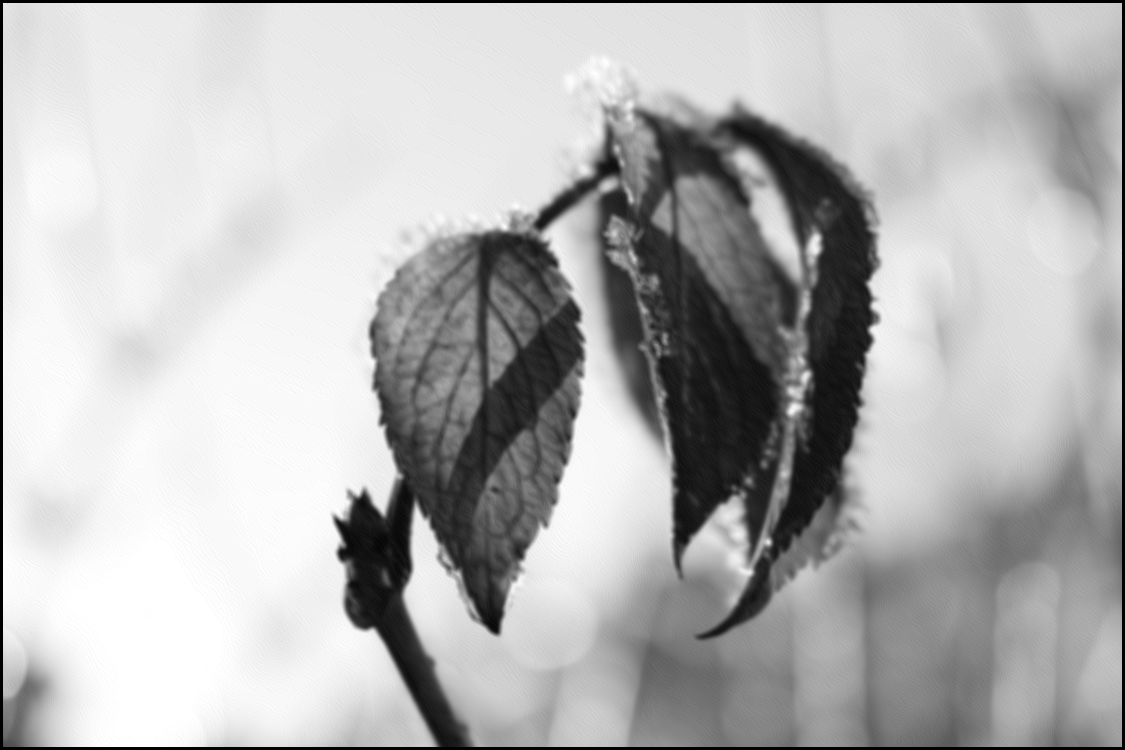
\includegraphics[width=\linewidth]{../output/neu2_output_18k_alpha0005.png}
  \caption{$\alpha=0.005$}
  \label{fig:bilda6}
\end{figure}

\begin{figure}
  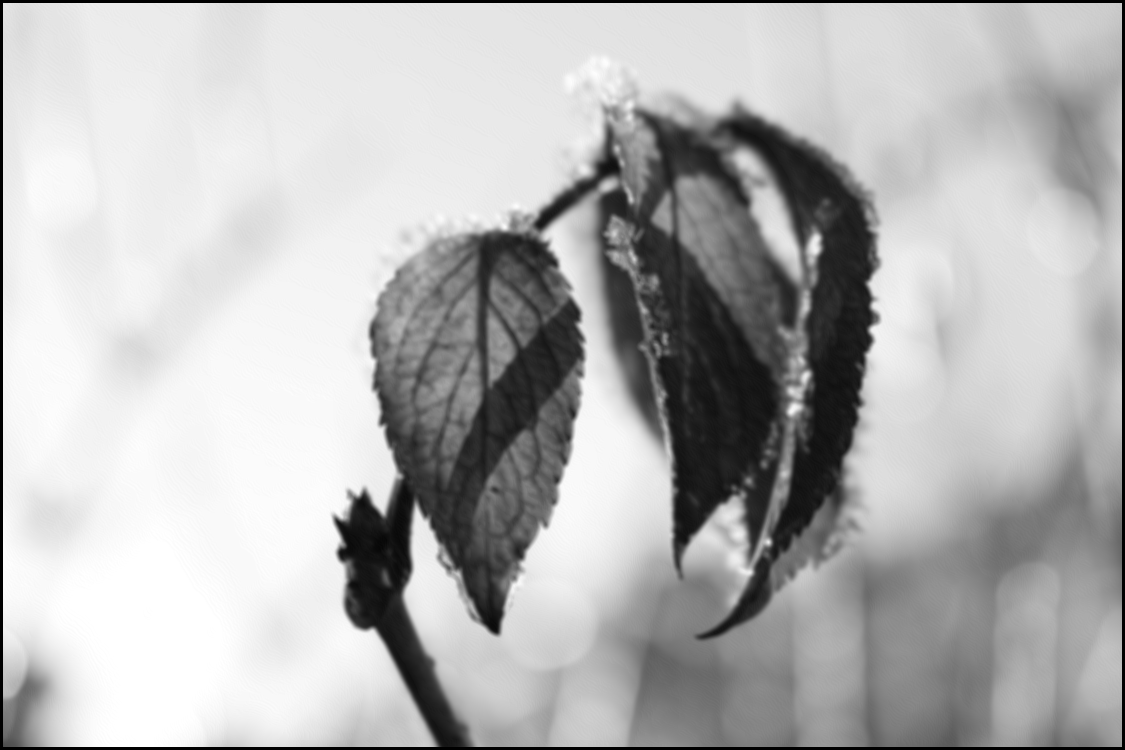
\includegraphics[width=\linewidth]{../output/neu2_output_18k_alpha00025.png}
  \caption{$\alpha=0.0025$}
  \label{fig:bilda7}
\end{figure}

\begin{figure}
  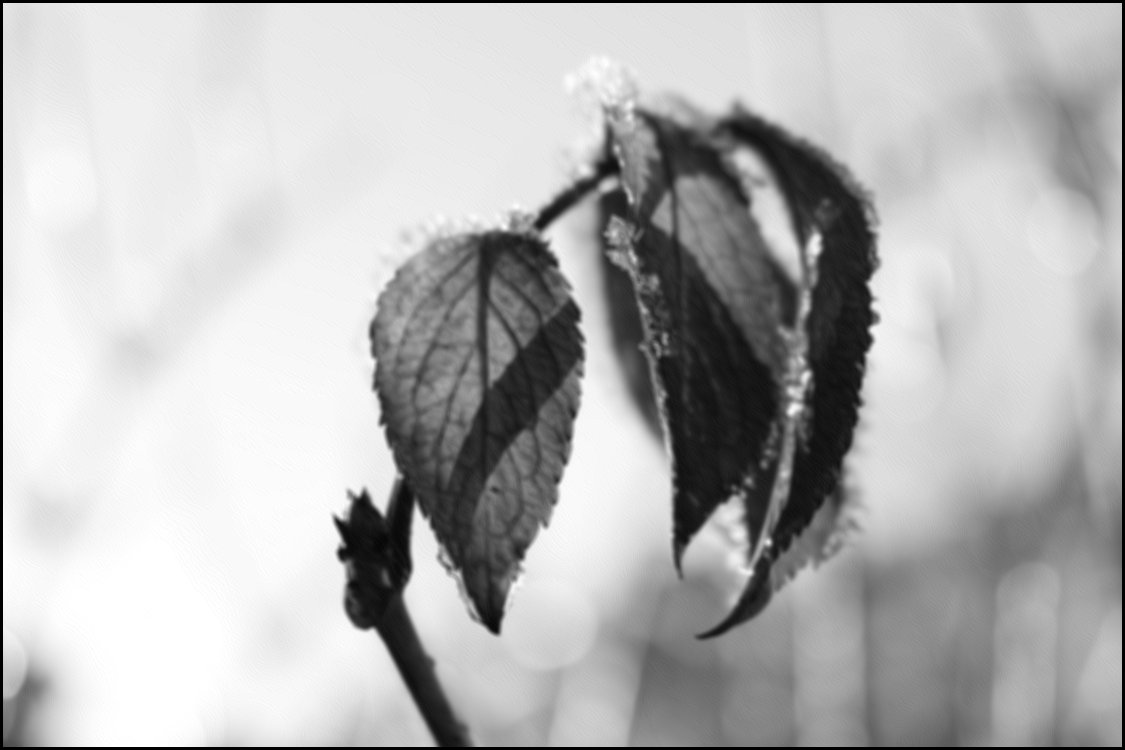
\includegraphics[width=\linewidth]{../output/neu2_output_18k_alpha000375.png}
  \caption{$\alpha=0.00375$}
  \label{fig:bilda8}
\end{figure}

% \bibliographystyle{alpha} verwendet Kuerzel aus Autorennamen und Jahreszahl
% \bibliographystyle{abbrv} verwendet numerische Referenzen
%\bibliographystyle{abbrv}
% Hier die *.bib-Datei angegeben, die verwendet werden soll! An dieser Stelle wird
% jetzt das Literaturverzeichnis erstellt.
%\bibliography{literatur.bib}


\end{document}